\section{Our Approach}
\label{sec:program:solution}

In this section, we first present our approach with the \texttt{mutual-sum} example (\Cref{sec:program:solution:mutsum}).
To the best of our knowledge, our framework is the first, in the context of \cc{}, that is capable of verifying the \emph{mutually recursive} modules.
Then, we point out that our approach does not suffer from aforementioned problems in \Cref{sec:program:problem} while supporting modular reasoning principle (\Cref{sec:program:solution:advantages}).
Additionally, we verify \texttt{utod}, \cc{}'s internal handwritten assembly function whose behavior is axiomatized, and show that such axioms can be removed (\Cref{sec:program:solution:utod}).
Finally, we report their verification efforts (\Cref{sec:program:solution:evaluation}).

\subsection{Verification of \texttt{mutual-sum}}
\label{sec:program:solution:mutsum}
\begin{figure}[t]
\makebox[\linewidth]{\makebox[1.1\linewidth]{
\begin{minipage}{1.1\linewidth}
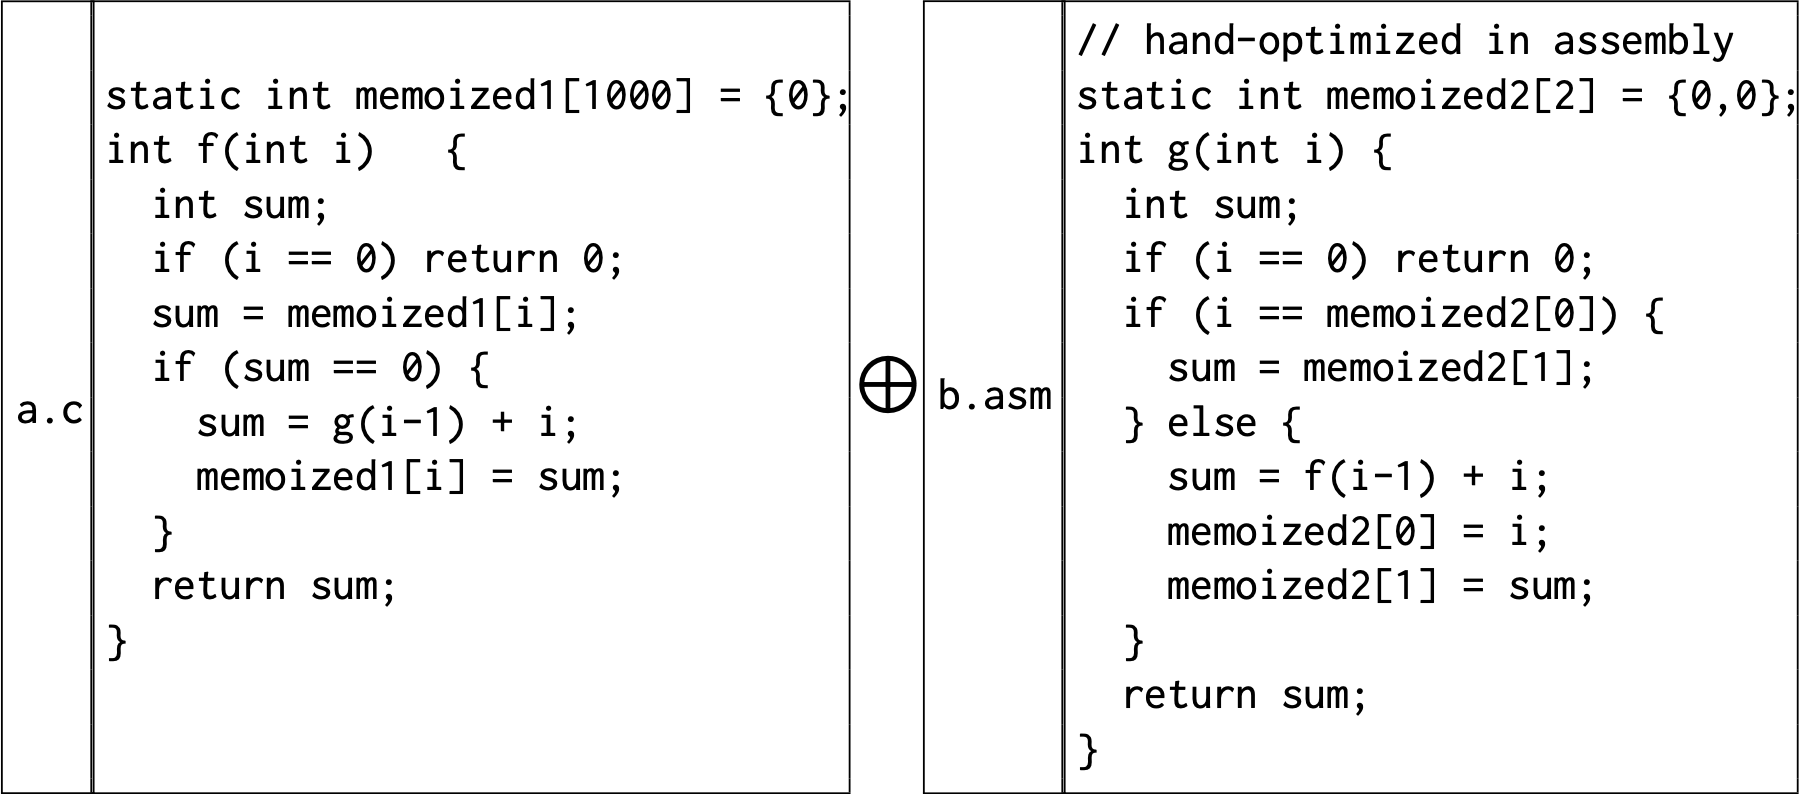
\includegraphics[width=1\linewidth]{images/mutsum1.png}
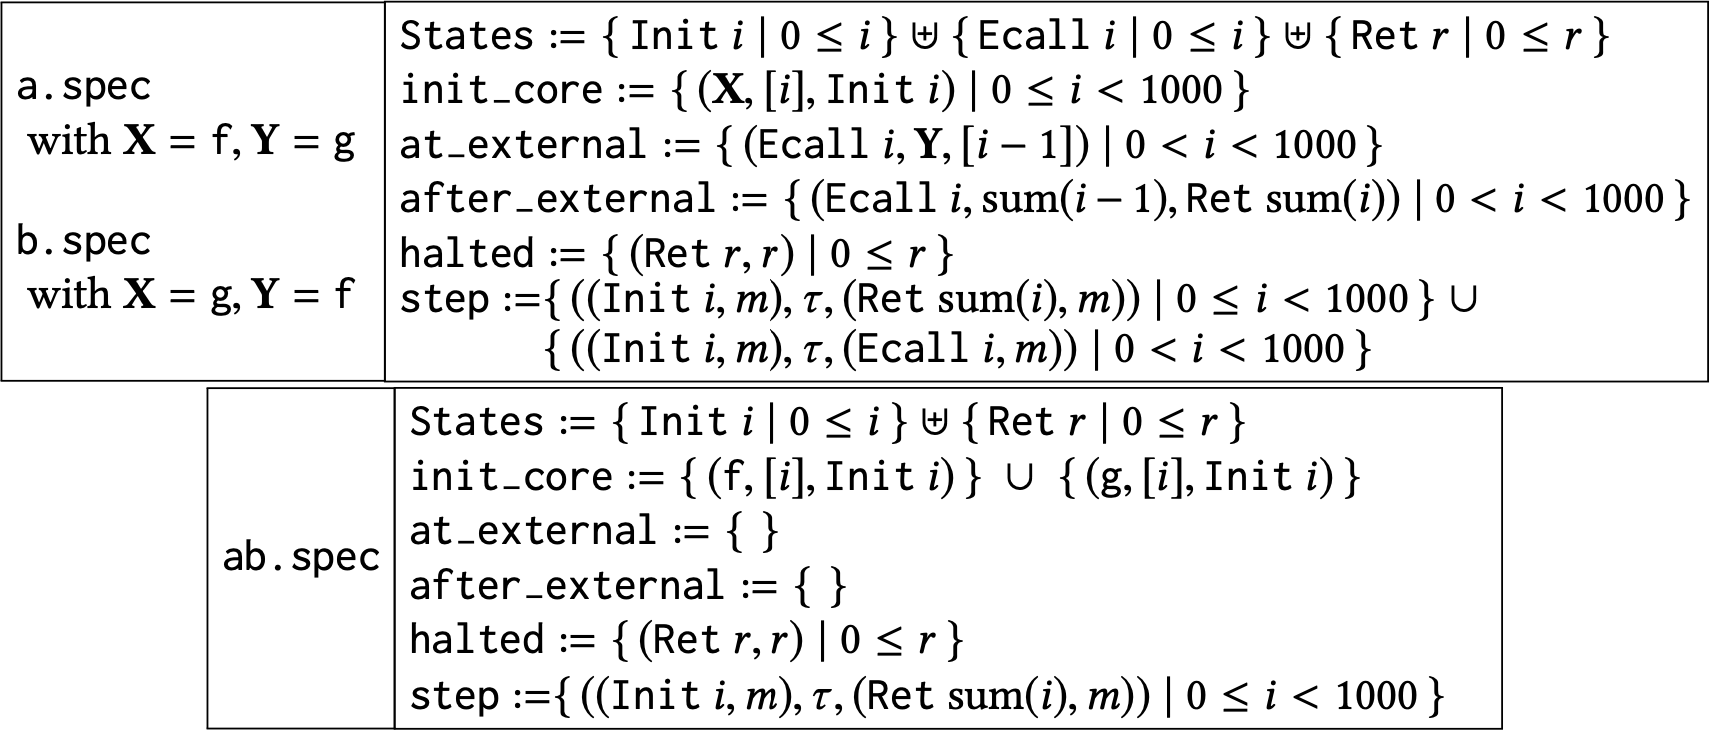
\includegraphics[width=1\linewidth]{images/mutsum2.png}
\end{minipage}
}}
\label{fig:modulelocal}
\end{figure}

\Cref{fig:modulelocal} shows a C module, \texttt{a.c}; a handwritten
assembly module, \texttt{b.asm} (presented in C syntax for
readability); their open specification modules, \texttt{a.spec} and
\texttt{b.spec}; and the combined closed specification module
\texttt{ab.spec}.  Both functions \texttt{f} in \texttt{a.c} and
\texttt{g} in \texttt{b.asm} mutually recursively compute the
summation from $0$ up to the given argument integer $i$ (denoted
$\mathrm{sum}(i)$), performing different memoization optimizations.
The function \code{f} memoizes the result of \code{f(i)} in the static
variable \code{memoized1[i]}, which is initialized with zero
representing invalid value.  The function call \code{f(i)} first reads
the memoized value, and returns it if it is valid; otherwise, it
calculates, memoizes, and returns \code{g(i-1)}, expected to be
$\mathrm{sum}(\code{i}-1)$, plus \code{i}.  On the other hand, the
function \code{g} memoizes only the result of the latest call
\code{g(i)} with the index \code{i}, where \code{memoized2[0]} =
\code{i} and \code{memoized2[1]} = \code{g(i)}.  The code of \texttt{g}
is self-explanatory under the assumption that the call \code{f(i-1)}
returns $\mathrm{sum}(\code{i}-1)$.

%% we have $\code{g(memoized[0])} = \code{memoized[1]}$.
%% The function \code{g(i)} is the same with
%% \code{f(i)}, except for memoization scheme, the callee of recursion,
%% and the language.

%% Our framework is flexible on the choice of languages to the degree that a module's (open)
%% specification can be represented as another module written in Coq's Gallina language.  Such
%% specification module facilitates modular verification of multi-language programs, as illustrated in
%% the example presented in \Cref{fig:modulelocal}.

%% Both of the function \code{f(i)} in the module \code{a.c} and \code{g(i)} in \code{b.asm} compute
%% $\textrm{sum}(\code{i})$, which is the summation from 1 to \code{i}, but with memoization and mutual
%% recursion on each other.\footnote{The module \code{b.asm} is written in hand-optimized assembly, but
%%   for presentational purposes we present it in C syntax.}  The module \code{a.c} memoizes the result
%% of \code{f(i)} in \code{memoized[i]}, which is initialized with zero representing invalid value.
%% The function \code{f(i)} first reads the memoized value, and returns it if valid; otherwise, it
%% calculates, memoizes, and then returns the summation of \code{g(i-1)}---which is expected to be
%% $sum(\code{i-1})$---and \code{i}.  On the other hand, \code{b.asm} memoizes only one result of
%% \code{g()}: we have $\code{g(memoized[0])} = \code{memoized[1]}$.  The function \code{g(i)} is the
%% same with \code{f(i)}, except for memoization scheme, the callee of recursion, and the language.


The open specification modules \texttt{a.spec} and \texttt{b.spec} are
the same except that the names of the internal and external functions
are swapped. This is natural because the two functions \code{f} and
\code{g} compute the same summation. The open specification
\texttt{a.spec} is an abstract, nondeterministic, version of the
function \texttt{f} in \texttt{a.c} including all the observable
behaviors of \texttt{f}.  It has three kinds of states,
$\code{Init}~i$, $\code{Ecall}~i$ and $\code{Ret}~r$, representing the
initial state with argument $i$, the call state executing
$\code{g}(i-1)$, and the halt state returning $r$, respectively. Then
\code{init\_core} starts with $\code{Init}~i$ when \texttt{f} is
invoked with argument $i$ if $0 \le i < 1000$, otherwise UB;
\code{at\_external} recognizes $\code{Ecall}~i$ as the state invoking
\texttt{g} with $i-1$; \code{after\_external} transitions
from $\code{Ecall}~i$ to $\code{Ret}~\mathrm{sum}(i)$ only
when the return value from the external call $\texttt{g}(i-1)$
is $\mathrm{sum}(i-1)$, otherwise UB, which
means that this module gives a conditional specification under the
assumption that $\texttt{g}(i)$ returns $\mathrm{sum}(i)$;
\code{halted} recognizes $\code{Ret}~r$ as the halted state returning
$r$; and finally $\code{step}$ transitions from $\code{Init}~i$ to
either $\code{Ret}~\mathrm{sum}(i)$ or $\code{Ecall}~i$
nondeterministically (without updating the memory), where the former
abstracts reading from memoization and the latter recursively
computing the sum. The same applies to \texttt{b.spec}.
Finally, the combined specification \code{ab.spec} does not make any
external function call and simply returns the summation.

Then, we perform our verification as follows.
First, we prove $\texttt{a.spec} \rusc_\rels \texttt{a.c}$
using memory injections with the following invariant:\\
%% \[
\mbox{}\hfill$\forall 0 \le i < 1000,~
\code{memoized1}[i] = 0 \lor \code{memoized1}[i] = \mathrm{sum}(i)~.$\hfill\mbox{}
%% \]
\\
Second, we prove $\texttt{b.spec} \rusc_\rels \texttt{b.asm}$
using memory injections with the following invariant:\\
%% \[
\mbox{}\hfill$
\exists 0 \le i < 1000,~
\code{memoized2}[0] = i \land \code{memoized2}[1] = \mathrm{sum}(i)~.
$\hfill\mbox{}
%% \]
\\
Finally, we prove $\texttt{ab.spec} \rusc_\rels \texttt{a.spec} \llink
\texttt{b.spec}$ using the memory identity.
\revision{Note that $\rels$ is the set containing open simulations with the three memory relations
  used in the above verification
  (\ie memory injections with the two invariants above and the memory identity).}

%% The module \code{ab.spec} represents a specification module for $\code{a.c} \llink \code{b.asm}$.
%% The specification essentially says \code{f(i)} and \code{g(i)} returns $sum(\code{i})$ if
%% $0 \le \code{i} < 1000$; otherwise, the behavior is undefined.  Note that the condition on \code{i}
%% comes from the fact that a bigger \code{i} causes buffer overrun at the access to \code{memoized[i]}
%% in \code{f(i)}.  Concretely, \code{ab.spec} has two kinds of states: \code{Init i} representing the
%% initial state with argument \code{i}, and \code{Ret res} representing the halted state with result
%% \code{res}; the module initializes a core with the initial state \code{Init i} when \code{f(i)} or
%% \code{g(i)} is invoked; an initial state \code{Init i} transitions to a return state \code{Ret
%%   $sum(\code{i})$} if $0 \le \code{i} < 1000$; and the module invokes no external function calls.

%% The verification of \code{a.c} and \code{b.asm} amounts to proving
%% $\beh{\texttt{ab.spec}} \supseteq \beh{\texttt{a.c} \llink \texttt{b.asm}}$, which comes from
%% linking the following verifications:
%% \[
%% \begin{array}{c}
%% \texttt{a.spec} \rusc_\rels \texttt{a.c}\quad
%% \texttt{b.spec} \rusc_\rels \texttt{b.asm}
%% \\
%% \texttt{ab.spec} \rusc_\rels \texttt{a.spec} \llink \texttt{b.spec}
%% \end{array}
%% \]
%% where $\rusc_\rels$ is the RUSC relation for a suitable set, $\rels$, of module relations, and
%% \code{a.spec} and \code{b.spec} are themselves (open) specification modules for \code{a.c} and
%% \code{b.asm}, respectively.  The specification module \code{a.spec} essentially says \code{f(i)},
%% provided that \code{i} is in a valid range, either $(i)$ returns $sum(\code{i})$; or $(ii)$ invokes
%% an external call \code{g(i-1)}, receives $sum(\code{i}-1)$ as a result, and then returns
%% $sum(\code{i})$.  To model the interaction with the external function call to \code{g(i-1)}, the
%% specification module has a state, \code{Ecall i}, that represents the call to \code{g(i-1)}.
%% Crucially, If the call does not return $sum(\code{i-1})$, the behavior is undefined.  The
%% specification module \code{b.spec} is the same with \code{a.spec}, except that \code{f} and \code{g}
%% are switched.

%% Verifications of $\texttt{a.spec} \rusc_\rels \texttt{a.c}$ and
%% $\texttt{b.spec} \rusc_\rels \texttt{b.asm}$ require module-local invariants, because the memoized
%% values in \code{memoized} should be private, as they exist only in the target, but they may be
%% changed during an external function call via mutual recursion.  As the module-local invariant, we
%% require that memoized values, if valid, are indeed correct.  On the other hand, verification of
%% $\texttt{ab.spec} \rusc_\rels \texttt{a.spec} \llink \texttt{b.spec}$ does not require module-local
%% invariants and any other complications from programming language semantics, but require reasoning
%% about multiple modules.

%% Specification module not only facilitates modular verification of multi-language programs, thereby
%% reducing the total verification cost, but also enables verification of handwritten assembly
%% functions whose correctness is axiomatized in \cc{}, reducing its trusted computing base (TCB).  See
%% \Cref{sec:utod-verification} for details.







\subsection{Advantages}
\label{sec:program:solution:advantages}
Our approach does not suffer from aforementioned problems in \Cref{sec:program:problem} while supporting modular reasoning principle (\Cref{sec:program:solution:advantages}).

First and foremost, by passively modeling the expected behavior of other modules with UB, we don't have any circularity in our reasoning.
Therefore, we don't need step-index so our specification is clean and easy to understand.
Furthermore, as our specification is written in an operational semantics, it can even be executed and tested.
It is very important to have a reliable and understandable specification, perhaps as important as the verification itself, and testing is widely adopted as a tool to establish such trust.
%
Second, we trivially support total correctness because the notion of behavior is termination-sensitive and we prove behavioral refinement.
%
Third, we don't impose any restriction on the client module because RUSC quantifies over an arbitrary context.
%
Finally, our specification module can trigger events just as C and assembly modules do, so we can definitely give a REPL-like specification.
Note that while we give terminating specification for terminating implementations and reactive (non-terminating and consistently communicating with outside world, like REPL) specification for reactive modules,
their correctness are all expressed in simple RUSC relation. This is in contrast with where they define Hoare triple for partial correctness and total correctness separately, and these two are not coexist.
















\subsection{Verification of \texttt{utod}}
\label{sec:program:solution:utod}
\verb|__compcert_i64_utod| (\Cref{fig:utod} - (d)) is one of the \cc{}'s internal handwritten
assembly functions, which converts \verb|unsigned long| to
\verb|double| by utilizing architecture-specific instructions like
\verb|cvtsi2sdq|.
Note that the call to this assembly function is introduced during compilation passes; for example a source program purely written in C (\Cref{fig:utod} - (a)) is translated to \verb|__compcert_i64_utod| (\Cref{fig:utod} - (b)).
In order to justify this translation, \cc{} currently axiomatizes the behaviors of such runtime libraries as described in \Cref{fig:utod} - (c).

\begin{figure}[t]
%% \makebox[\linewidth]{\makebox[1.1\linewidth]{
%% \begin{minipage}{1.1\linewidth}
%% 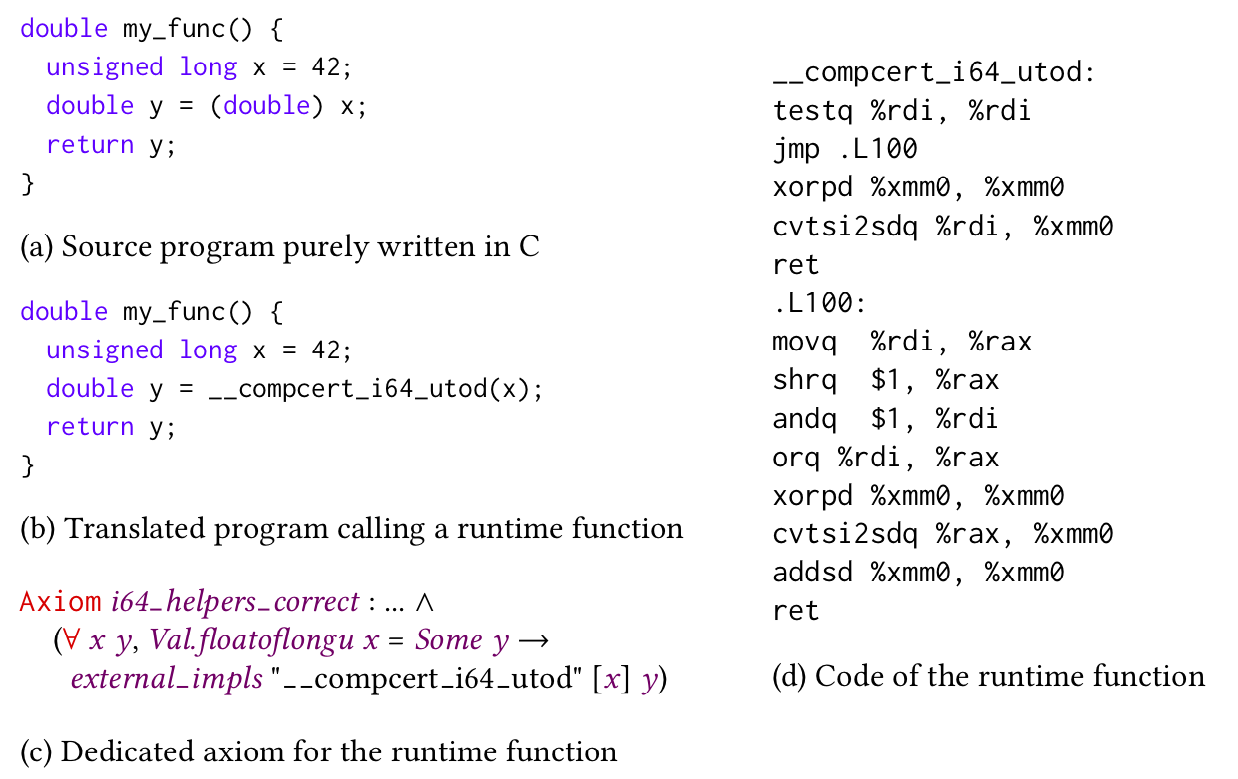
\includegraphics[width=1\linewidth]{images/utod.png}
%% \end{minipage}
%% }}
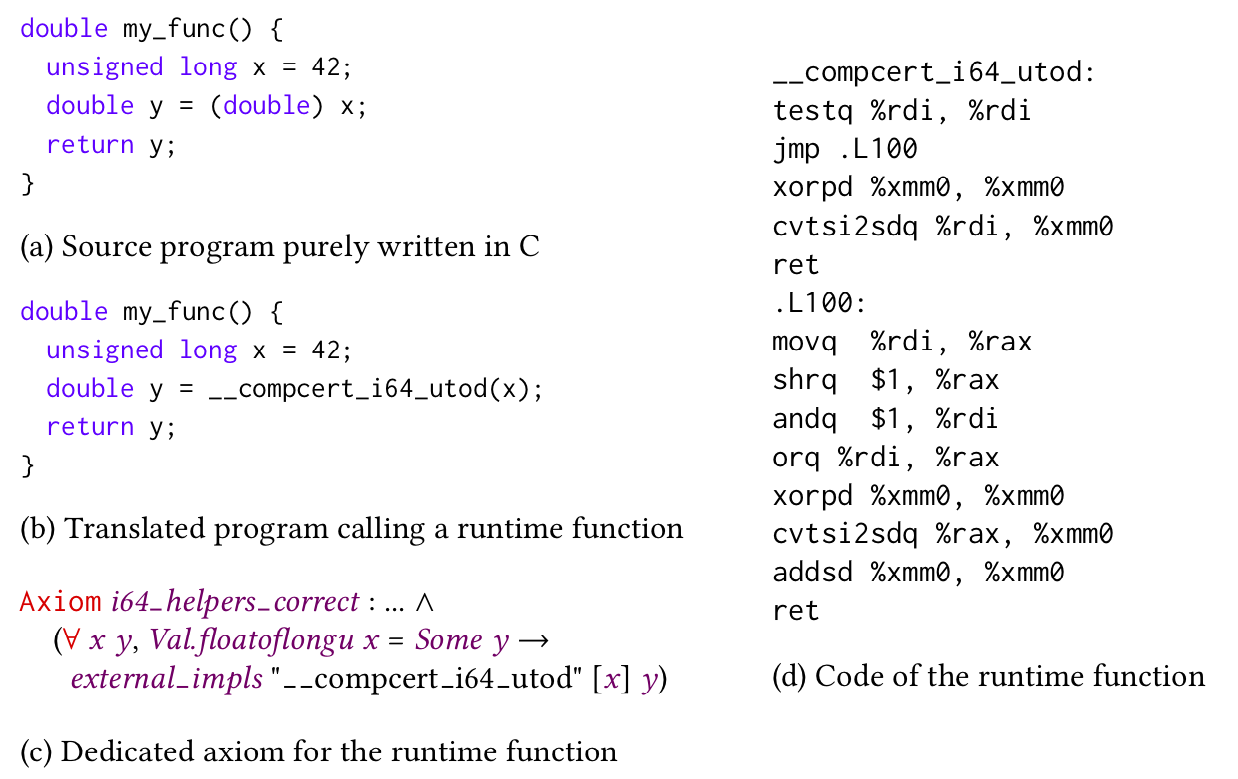
\includegraphics[width=1\linewidth]{images/utod.png}
\caption{Verification of \texttt{utod}}
\label{fig:utod}
\end{figure}



%% \[
%% \begin{minipage}{\textwidth}
%% \begin{coqdoccode}
%% \coqdocnoindent
%% \coqdockw{Axiom} \coqdoccst{i64\_helpers\_correct} : ... \ensuremath{\land}\coqdoceol
%% \coqdocindent{0.5em}
%% (\coqdockw{\ensuremath{\forall}} \coqdocvar{x} \coqdocvar{z}, \coqdocmod{Val}.\coqdoccst{floatoflongu} \coqdocvar{x} = \coqdocconstr{Some} \coqdocvar{z} \ensuremath{\rightarrow}
%% \coqdoccst{external\_implements} "\_\_compcert\_i64\_utod" \coqdoccst{sig\_l\_f} [\coqdocvar{x}] \coqdocvar{z})
%% \end{coqdoccode}
%% \end{minipage}
%% \]

We demonstrate that such axioms can be essentially removed in \ccm{} by proving the axiom for \verb|__compcert_i64_utod|.
We first turn the axiom for \verb|__compcert_i64_utod| into a specification module
and then establish an open simulation with memory injections between the assembly module containing \verb|__compcert_i64_utod| and the specification module.

\subsection{Verification Effort}
\label{sec:program:solution:evaluation}

\Cref{table:evaluation-program} shows SLOC for the program verification examples presented above.

Pass proofs (establishing open simulation between the specification and the implementation module) are mostly mechanical and tedious.
They mostly consist of executing C (or assembly) semantics step-by-step, doing simple reduction on local environment (or register state), and applying memory related lemmas appropriately.
Note that all of these are shared pattern among general C (or assembly) program verification.
We didn't do any proof automation at all, so there is big room for improvement.

For ``The Rest'', \texttt{mutual-sum} and \texttt{utod} have quite different reasons for their SLOC.
In \texttt{utod}, the whole SLOC is about proving self-relatedness of the specification module.
Recall that we verified self-relatedness for arbitrary C and assembly modules but not for arbitrary specification modules (it is not true).
In \texttt{mutual-sum} however, about 1,089 SLOC are from $\texttt{ab.spec} \rusc_\rels \texttt{a.spec} \llink \texttt{b.spec}$.
As discussed above, the proof of this translation is mainly about termination which should (morally) be easy.
Main technical hassle that made this long SLOC is that we had to take unknown context into account.
Such reasoning can be made as a general purpose meta-theory.


%% As the verification of \code{mutual-sum} and \code{utod} show, directly proving open simulation between programs and specifications is costly. 
%% We believe that program logics like VST~\cite{VST} can be used to prove such simulation, which could significantly reduce the verification cost.



\begin{table}[t]
\centering
\caption{SLOC of additional developments}
\begin{tabu}{@{}l @{\;} |[1.25pt] @{\;} r @{\;} | @{\;} r @{\;}}
Portion                          & \texttt{mutual-sum} & \texttt{utod} \\
\hline
Pass Proofs                      & 3,088               & 361           \\
The Rest                         & 2,707               & 424           \\
Total                            & 5,795               & 785           \\
\end{tabu}
\label{table:evaluation-program}
\end{table}

















\hide{
Now we explain how we can apply RUSC to program verification with an example (\Cref{fig:program-verif}) where two mutually recursive modules $\texttt{f.c}$ and $\texttt{g.c}$ are verified against its specifications even in the presence of an unknown assembly module $\texttt{h.asm}$.

First, we write a specification as a {\it module}, not in C but in abstract mathematical state transition system. %%simpler, abstract
For an instance, if we have a C module computing Fibonacci number employing dynamic programming technique, its specification module directly returns $\mathrm{Fib}(\code{n})$ for an argument \code{n} where $\mathrm{Fib}$ is a Gallina function.
Existing works\cite{lorch:armada, jung:irisjfp, VST, gu:dscal} often take different choice with us, where they write specifications in a specific language, as a {\it Hoare triple}, or as a CAL.
We use state transition system because it is the most general form, and fortunately it is already supported in interaction semantics. %% TODO: compare with multi-language semantics?

Then, each implementation module (written in C or assembly) is verified against its specification module using open simulations, thus implying RUSC relation.
The challenge here is: How to utilize the specifications of other modules even though what we are proving is RUSC, which quantifies over an arbitrary context?
Our key idea is that, instead of directly assuming the specifications of other modules, we carefully massage each specification module with UB in order to give an illusion as if we are assuming specifications of other modules.
Specifically, $\texttt{f.spec}$ calls $\texttt{g}$ -- which can be an arbitrary function because we are proving under an arbitrary context -- and then check if $\texttt{g}$ returns the expected value. If so, it will proceed, but if not, it will trigger UB.
As a result, when verifying $\texttt{f.spec} \rusc_\rels \texttt{f.c}$ one needs to proceed the simulation proof only when $\texttt{g}$ behaves as expected, because otherwise the proof is trivial.
After each module's verification is over, we can {\it merge} these modules to form $\texttt{fg.spec}$ and remove the potential source of UB.
This way, we can handle cooperation among the modules naturally.

Finally, recall that RUSC lifts (almost) arbitrary open simulations.
Therefore, even though verifying $\texttt{f.c}$ againts $\texttt{f.spec}$ requires a specialized simulation, RUSC can ably support them.

\todo{say that termination proof and functional correctness proof is separated}







Our approach supports modular reasoning principle in the presence of mutual recursion, but does not suffer from aforementioned drawbacks.
%% Now, we will explain what our approach is
First, we write a specification as a {\it module}, not in C but in abstract mathematical state transition system. %%simpler, abstract
For an instance, if we have a C module computing Fibonacci number employing dynamic programming technique, its specification module directly returns $\mathrm{Fib}(\code{n})$ for an argument \code{n} where $\mathrm{Fib}$ is a Gallina function.
Then, each implementation module (written in C or assembly) is verified against its specification module using open simulations, thus implying RUSC relation.
The challenge here is: How to utilize the specifications of other modules even though what we are proving is RUSC, which quantifies over an arbitrary context?
Our key idea is that, instead of directly assuming the specifications of other modules, we carefully write each specification module to give an illusion as if we are assuming specifications of other modules.
Specifically, in $f_{spec}$, it calls $g$ and then check if $g$ returns the expected value. If so, it will proceed, but if not, it will trigger UB.
As a result, when verifying $f_{spec} \rusc_\rels f_{impl}$ one needs to proceed the simulation proof only when $g$ behaves as expected, because otherwise the proof is trivial.
Finally, after each module's verification is over, we can {\it merge} these modules to form $fg_{spec}$ and remove the potential source of UB.

%% 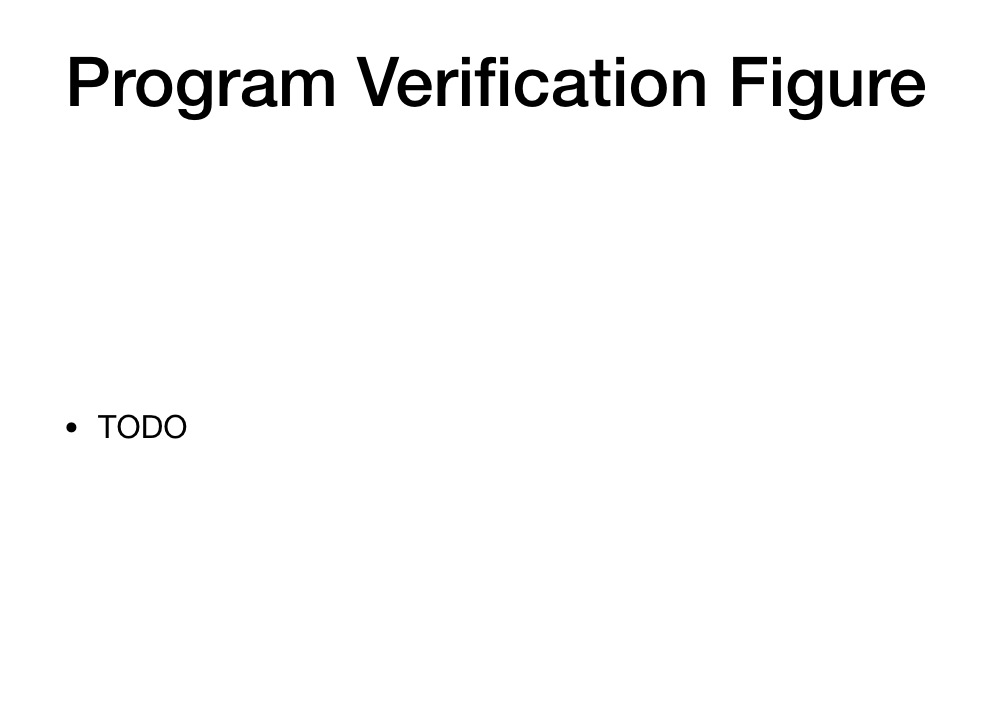
\includegraphics[width=0.6\linewidth]{fig-program-verif.png}

\noindent Now we explain why our approach does not suffer from the drawbacks.
First and foremost, by passively modeling the expected behavior of other modules with UB, we don't have any circularity in our reasoning. Therefore, we don't need step-index and can use RUSC framework without any problem.
Second, we trivially support total correctness because the notion of behavior is termination-sensitive.
Third, we don't impose any restrictions on the client module because RUSC quantifies over an arbitrary context.
}

%% \section{Comparison with Hoare Logic}
\label{sec:program:hoare}

%% \section{Future Works}
\label{sec:program:future}
%% automation 이야기... layered approach

%% \section{Background}
%% \label{sec:program:background}

%% \section{Problems}
%% \label{sec:program:problems}

%% \section{Solution}
%% \label{sec:program:solution}

